\section{
    Implemente no JFlap uma MT que reconheça a seguinte linguagem: \{cadeias binárias que não contenham a subcadeia 101\}
    }

\setlength{\parindent}{4em}
\setlength{\parskip}{0.5em}
\renewcommand{\baselinestretch}{1}

\begin{figure}[h]
    \centering
    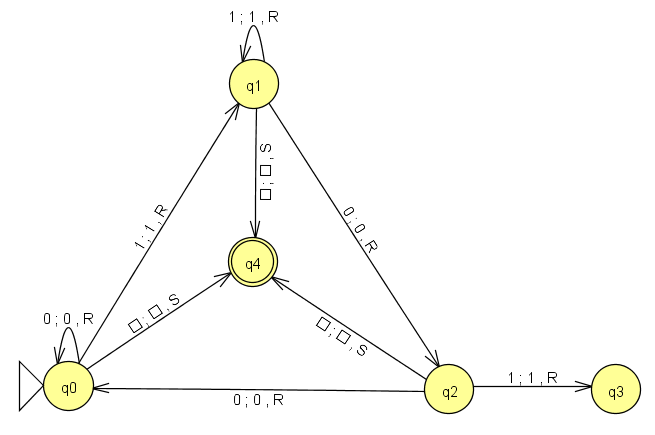
\includegraphics[width=0.65\textwidth]{mtex3.png}
    \caption{Máquina de Turing desenvolvida para o exercício no JFlap.}
    \label{fig:mtex3}
\end{figure}

\blindtext
